% Asset ID: AS1EquationsInequalitiesTikZ-002
% Source: CCEA AS1-AF-LO009; P1 Chapter 3 PDF quadratic inequalities section.
% Related lesson section: Core Theory: Quadratic Inequalities.
% Purpose: Clean sign/graph diagram for y = (x+5)(x-3).
\documentclass[tikz,border=8pt]{standalone}
\usepackage{amsmath}
\usepackage{tikz}
\usetikzlibrary{arrows.meta,patterns}
\begin{document}
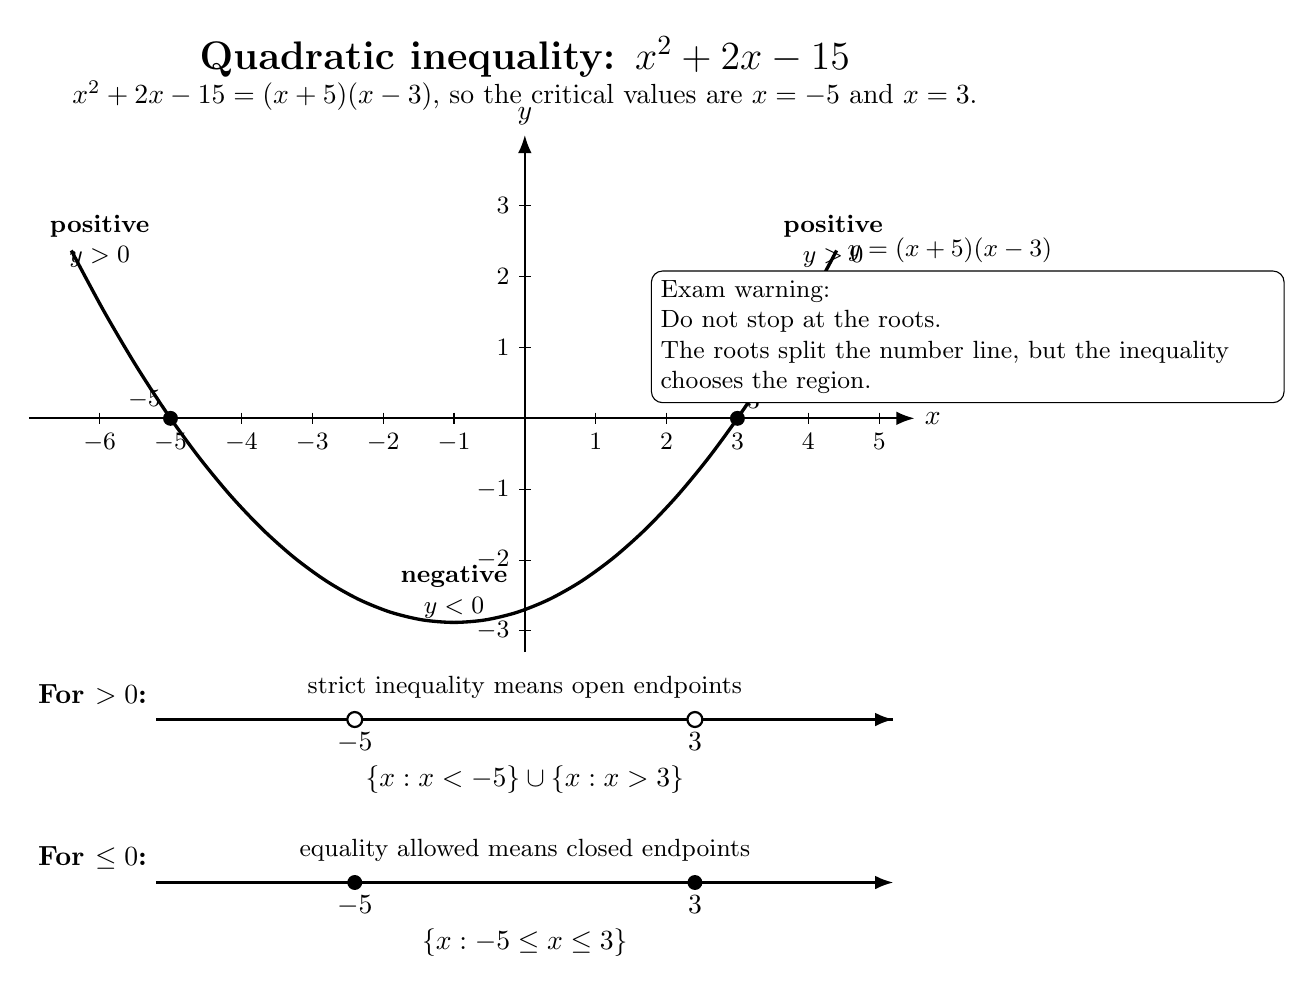
\begin{tikzpicture}[scale=0.9, >=Latex]
  \node[font=\Large\bfseries] at (0,5.1) {Quadratic inequality: $x^2+2x-15$};
  \node[font=\normalsize] at (0,4.55) {$x^2+2x-15=(x+5)(x-3)$, so the critical values are $x=-5$ and $x=3$.};
  \draw[->, thick] (-7,0) -- (5.5,0) node[right] {$x$};
  \draw[->, thick] (0,-3.3) -- (0,4.0) node[above] {$y$};
  \foreach \x in {-6,-5,-4,-3,-2,-1,1,2,3,4,5} \draw (\x,0.08) -- (\x,-0.08) node[below, font=\small] {$\x$};
  \foreach \y in {-3,-2,-1,1,2,3} \draw (0.08,\y) -- (-0.08,\y) node[left, font=\small] {$\y$};
  \node[font=\small\bfseries, align=center] at (-6,2.5) {positive\\$y>0$};
  \node[font=\small\bfseries, align=center] at (4.35,2.5) {positive\\$y>0$};
  \node[font=\small\bfseries, align=center] at (-1,-2.45) {negative\\$y<0$};
  \draw[domain=-6.4:4.4, smooth, variable=\x, very thick] plot ({\x},{0.18*(\x+5)*(\x-3)}) node[right, font=\small] {$y=(x+5)(x-3)$};
  \fill (-5,0) circle (3pt); \fill (3,0) circle (3pt);
  \node[above left, font=\small] at (-5,0) {$-5$}; \node[above right, font=\small] at (3,0) {$3$};
  \begin{scope}[shift={(0,-4.25)}]
    \node[font=\bfseries] at (-6.1,0.35) {For $>0$:};
    \draw[->, thick] (-5.2,0) -- (5.2,0);
    \draw[very thick] (-5.2,0) -- (-2.45,0); \draw[very thick] (2.45,0) -- (5.2,0);
    \draw[fill=white, thick] (-2.4,0) circle (3pt); \draw[fill=white, thick] (2.4,0) circle (3pt);
    \node[below] at (-2.4,-0.05) {$-5$}; \node[below] at (2.4,-0.05) {$3$};
    \node[font=\small] at (0,0.45) {strict inequality means open endpoints};
    \node[font=\bfseries] at (0,-0.85) {$\{x:x<-5\}\cup\{x:x>3\}$};
  \end{scope}
  \begin{scope}[shift={(0,-6.55)}]
    \node[font=\bfseries] at (-6.1,0.35) {For $\le 0$:};
    \draw[->, thick] (-5.2,0) -- (5.2,0);
    \draw[very thick] (-2.4,0) -- (2.4,0);
    \fill (-2.4,0) circle (3pt); \fill (2.4,0) circle (3pt);
    \node[below] at (-2.4,-0.05) {$-5$}; \node[below] at (2.4,-0.05) {$3$};
    \node[font=\small] at (0,0.45) {equality allowed means closed endpoints};
    \node[font=\bfseries] at (0,-0.85) {$\{x:-5\le x\le 3\}$};
  \end{scope}
  \node[draw, rounded corners, align=left, fill=white, text width=7.8cm, font=\small] at (6.25,1.15) {Exam warning:\\Do not stop at the roots.\\The roots split the number line, but the inequality chooses the region.};
\end{tikzpicture}
\end{document}
